\begin{figure}[!htp]
    \centering
    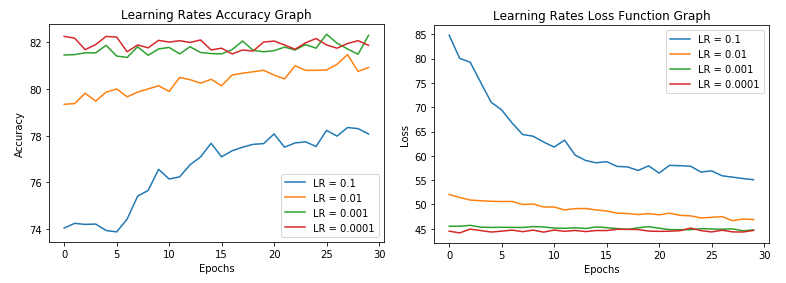
\includegraphics[width=15cm]{Images/lr.png}
    \caption{Variable Learning Rates}
    \label{fig:lrates}
\end{figure}

The figure \ref{fig:lrates} above shows that the model was trained for different learning rates as shown
in the legend of the figure \ref{fig:lrates} for thirty epochs or iterations. The outcome of the above test 
was that the model model accuracy of the model were increasing with decrease in the learning rates. 
The graph obtained shows that the model accuracy was proportional to the learning rate while using SGD optimiser. 
The figure \ref{fig:lrates} also shows the decline in the loss function for different learning rates in 
convolutional model trained with SGD optimiser. Therefore, the most optimal learning rate to train the convolutional network 
neural network was 0.1 and 0.001. During the experiments, it was observed that model with the lower the learning rate consumes more time in the 
process of training. Further model training experiments are peformed on 
learning rate of 0.01 to achieve the accuracy and realtive speed to train the model.
\pagebreak

\subsection*{Accuracy Results from Learning Rate experiments}

\begin{center}
    \begin{tabular} { | c | c | c | c | c |}
        \hline
        Training Time & Learning Rate & Test Accuracy & Epochs  & Optimiser\\ 
        \hline
        02:31:15 & 0.1 & 73.3\% & 140 & SGD \\ 
        \hline 
        02:32:52 & 0.01 & 81.01\% & 140 & SGD  \\
        \hline 
        02:33:00 & 0.001 & 69.75\% & 140 & SGD \\
        \hline
        02:33:22 & 0.0001 & 72.7\% & 140 & SGD \\
        \hline
        02:33:39 & 0.00001 & 72.7\% & 140 & SGD \\
        \hline
    \end{tabular}
\end{center}

The results presented above were evaluated on testing data and shows the 
direct relation of the time required to train convolutional neural network 
where decreasing learning rates requires more time to train models. These results 
are obtained by traing the model on Nvidia GTX-1080 gpu(graphical processing unit), training 
time might differ on different gpu based on it computational power.